\documentclass[a4paper,12pt]{article}
\usepackage{../../mypackages}
\usepackage{../../macros}


\usepackage{pgfplots}
    \pgfplotsset{
    compat=1.11,
  }

\setlength{\parindent}{0pt}


\begin{document}

\title{Chapitre 1 - Exercices}
\author{N. Bancel}

\maketitle

\section{Exercice 10}

\begin{figure}[H]
  \centering
  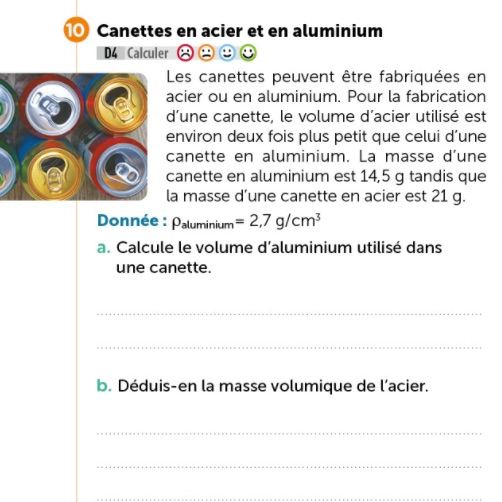
\includegraphics[width=0.5\linewidth]{exo_10.jpg}
  \caption{\label{} Exercice 10}
\end{figure}


\subsection{Question 1}

\textbf{Théorie} : 

\[
V_{\text{aluminium}} = \frac{m_{\text{aluminium}}}{\rho_{\text{aluminium}}}
\]

\textbf{Application numérique} : 

\[
V_{\text{aluminium}} = \frac{14.5}{2.7} = \SI{5.37}{\cubic\centi\meter}.
\]

\subsection{Question 2}

\textbf{Théorie} : 

\[
V_{\text{acier}} = \frac{V_{\text{aluminium}}}{2}
\]

\[
\rho_{\text{acier}} = \frac{2 \cdot m_{\text{acier}}}{V_{\text{aluminium}}}
\]

\textbf{Application numérique} : 

\[
\rho_{\text{acier}} = \frac{2 \cdot 21}{5.37} = \SI{7.82}{g\per\cubic\centi\meter}.
\]

Conversion en kg/L est équivalente (x1000 en haut, x1000 en bas) - c'est cohérent

\end{document}


